Consider the implicit Runge-Kutta method

$$U^*=U^n+\frac{h}{2}f(t_n+\frac{h}{2},U^*)$$
$$U^{n+1}=U^n+hf(t_n+\frac{h}{2},U^*)$$

a. Determine the order of accuracy of this method.\\
b. Determine the absolute stability region. Is it A-stable? L-stable?\\
c. Use this method to solve the initial value problem $u'(t)=2(t+1)$, $u(1)=3$\\

\begin{solution}\renewcommand{\qedsymbol}{}\ \\
    a. Using $f(u)=\lambda u$ on $U^*$ first gives us

    $$u_*=u_n+\frac{h}{2}\lambda u_*$$

    So,

    $$u_*=\frac{2u_n}{2-h\lambda}$$

    Plugging this into the corrector yields

    $$U^{n+1}=U^n+hf(t_n+\frac{h}{2},\frac{2U^n}{2-z})\;\;z=h\lambda$$

    Again using $f(u)=\lambda u$, we get

    $$u_{n+1}=u_n+h\lambda\frac{2u_n}{2-z}$$

    Whence,

    $$\frac{u_{n+1-u_n}}{h}=\lambda\frac{2u_n}{2-z}$$

    Hence, our truncation error becomes

    $$\tau=\frac{u_{n+1-u_n}}{h}-\lambda\frac{2u_n}{2-z}=\frac1hu_{n+1}-\frac1hu_n-
    \lambda\frac{2u_n}{2-z}$$

    Expanding $u_{n+1}$ about $u_n$ gives us

    $$\tau=\frac1h(u_n+hu_n'+\frac{h^2}{2}u_n''+\mathcal{O}(h^3))-\frac1hu_n-
    \lambda\frac{2u_n}{2-z}$$
    $$=u_n'+\frac{h}{2}u_n''+\mathcal{O}(h^2)-\lambda\frac{2u_n}{2-z}$$

    Using $u'=\lambda u$, we have

    $$\tau=\lambda u_n+\frac{h\lambda^2}{2}u_n-\lambda\frac{2u_n}{2-z}+\mathcal{O}(h^2)$$
    $$=-\frac{h\lambda^2u_n}{2-z}+\frac{h\lambda^2}{2}u_n+\mathcal{O}(h^2)$$
    $$=-\frac{h\lambda^2u_n}{2-z}+(\frac{1-\frac12h\lambda}{1-\frac12z})\frac{h\lambda^2}{2}u_n+
    \mathcal{O}(h^2)$$
    $$=-\frac{\frac{1}{2}z^2\lambda}{2-z}u_n+\mathcal{O}(h^2)$$

    Thus, we see that this implicit Runge-Kutta method is of the order of $h^2$\\

    b. From above, we see that $R(z)=1+\frac{2z}{1-z}=\frac{2+z}{2-z}$. So, the stability region is the
    set $\{z\in\mathbb{C}|\;|\frac{2+z}{2-z}|\leq1\}$. Clearly, $\lim_{z\rightarrow\infty}|R(z)=1|$, so
    this method is not L-stable. We also have that
    $R^{-1}(e^{i\theta})=\frac{2(e^{i\theta}-1)}{e^{i\theta}+1}$ and since for all $\theta\in[0,2\pi]$,
    $Re(R^{-1})$ is defined, we have that the method is A-stable.\\

    c. Since the ODE in question is only dependent on $t$, we have that the code comes down to an
    explicit single step method. The code is implemented below and just as above in problem 2, the true
    solution is $u(t)=t^2+2t$.

    \begin{center}
    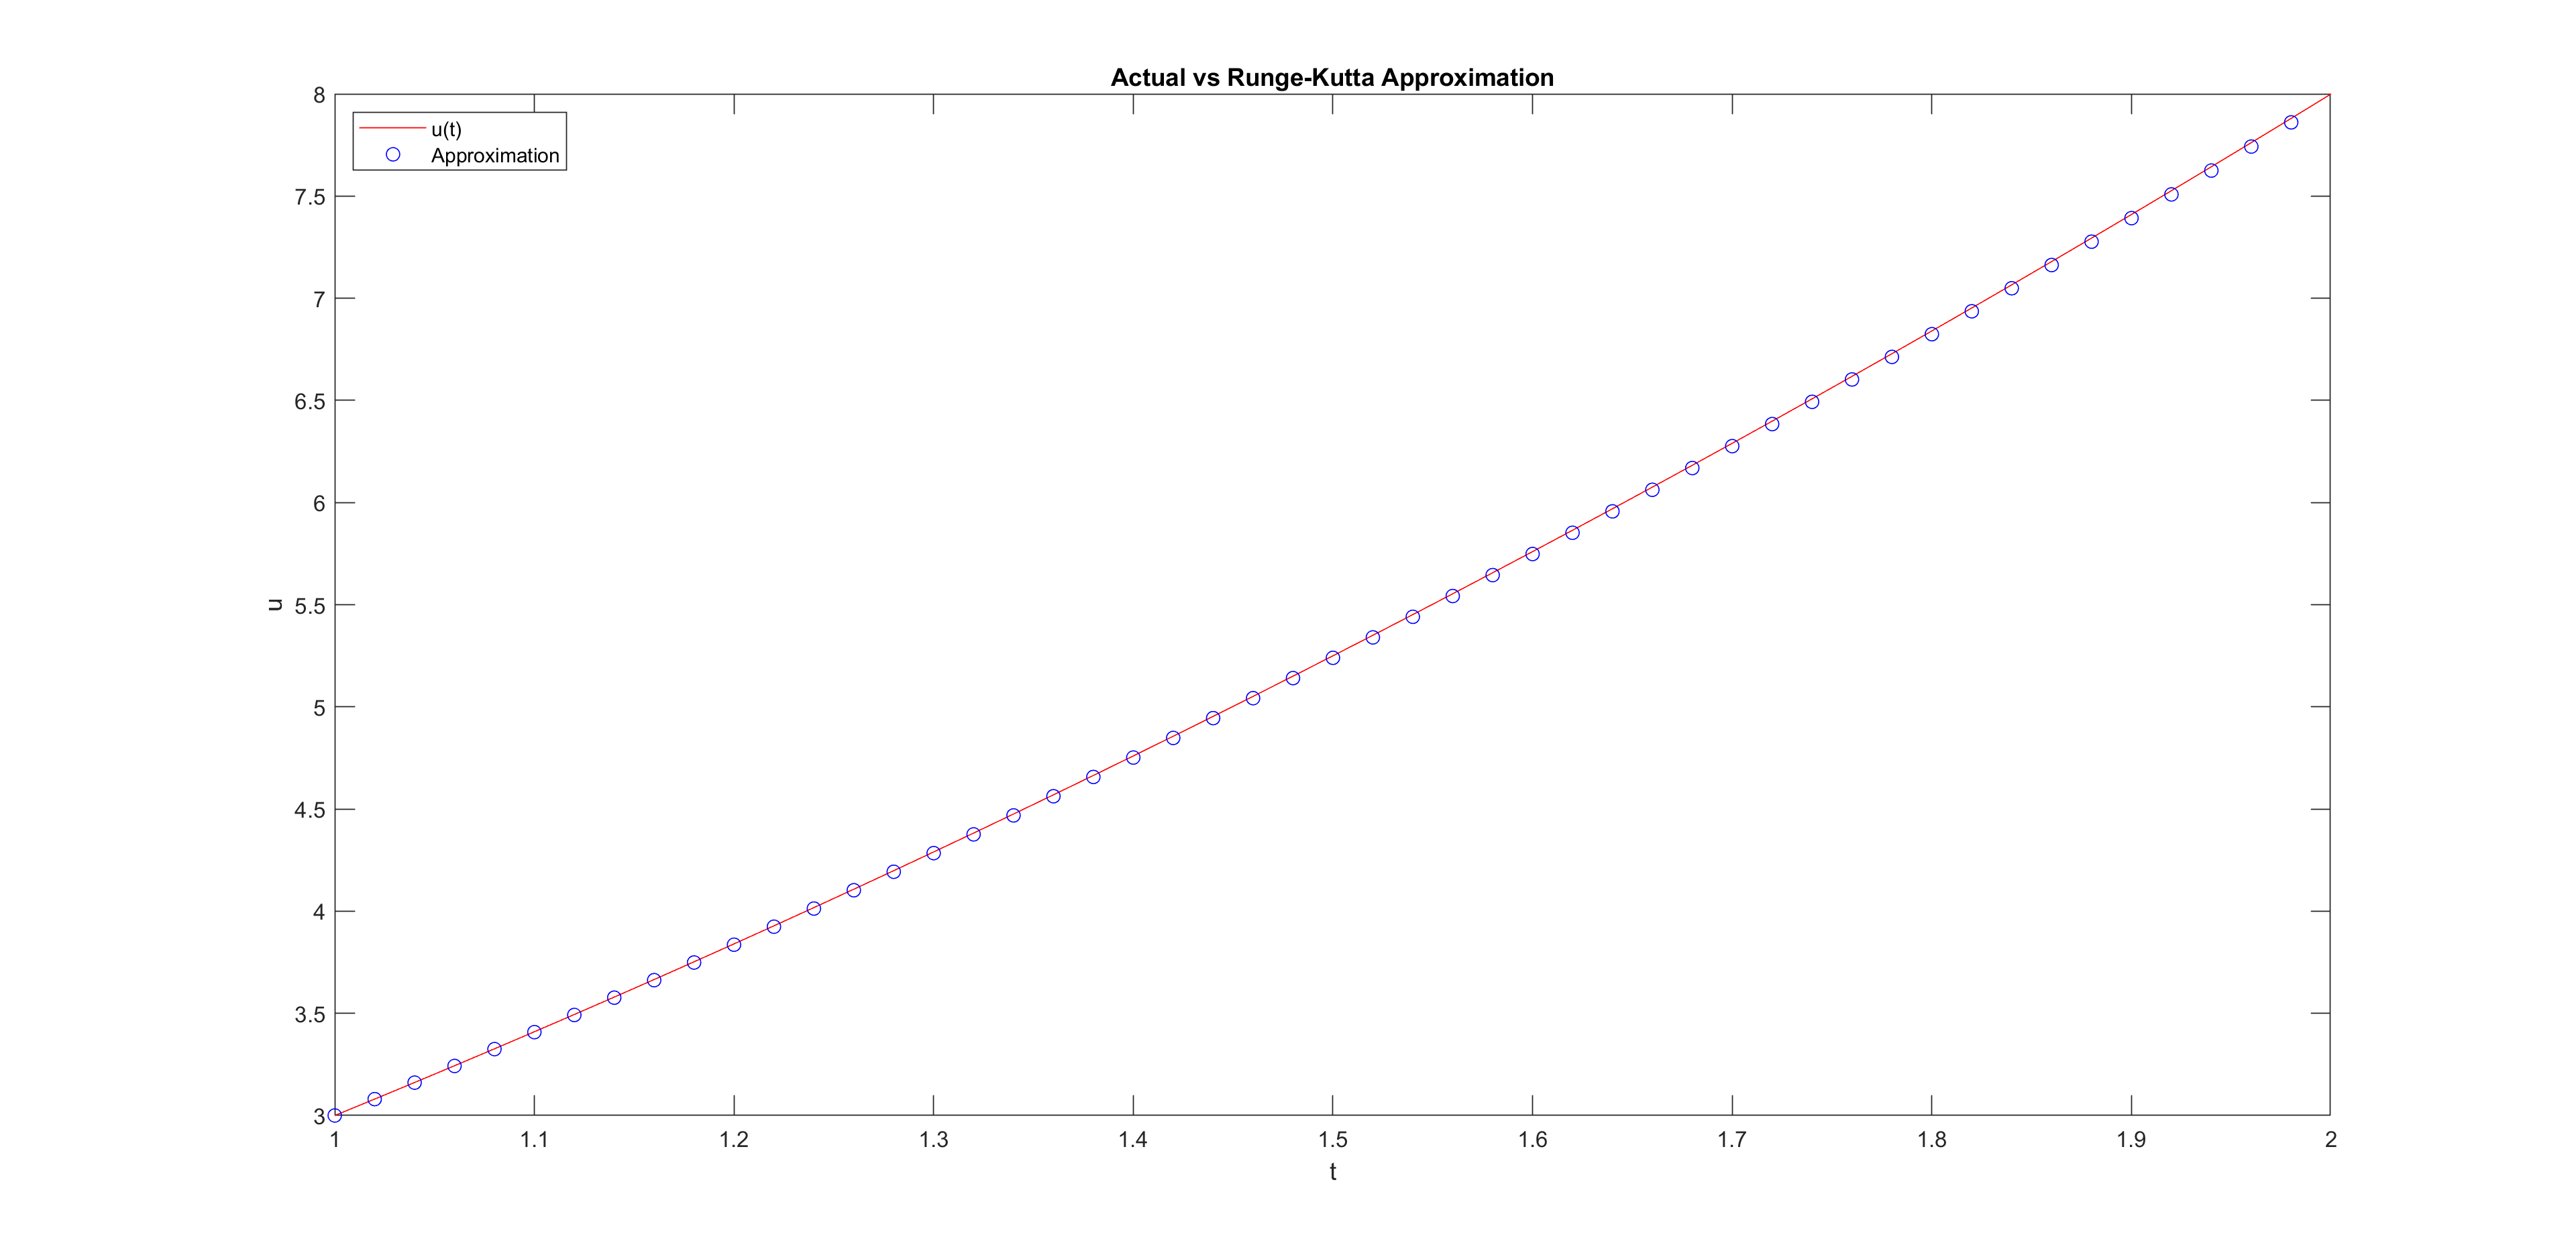
\includegraphics[scale=0.15]{3.PNG}
    \end{center}

\end{solution}

\newpage
\lstinputlisting{num3.m}